\subsection{Aggregation and time windows}
\label{sec:r-aggregation}

% Owner: A
\paragraph{Contact and messaging networks (PS, CM).}
\outline{Which conclusions are stable under window choice, and over which
$\Delta t$ range?}
\expect{[Expected] Density and clustering of the snapshots rise quickly with
$\Delta t$ and approach the aggregate only for windows comparable to the whole
observation period. The giant component of short-window snapshots is small, and
percolates at a window that is much shorter for CM than for PS because PS has a
daily rhythm (lessons, breaks). Conclusions about ``the'' clustering or density of
the network therefore depend strongly on $\Delta t$.}

\begin{figure*}[t]
\centering
\figph{0.32\textwidth}{3.6cm}{density vs.\ $\Delta t$\\(PS, CM)}\hfill
\figph{0.32\textwidth}{3.6cm}{clustering vs.\ $\Delta t$\\(PS, CM)}\hfill
\figph{0.32\textwidth}{3.6cm}{giant component vs.\ $\Delta t$\\(PS, CM)}
\caption{Structural metrics of snapshots as functions of the window length
$\Delta t$; dashed lines show the static aggregate. (Placeholder.)}
\label{fig:agg-window}
\end{figure*}

% Owner: B
% Owner: B -- measured CIT contribution only.
\paragraph{Citation network (CIT).}
In 2020, annual and cumulative graphs on the same 19,150 born nodes contain
1,450 and 73,269 citations. Mean total degree is 0.151 versus 7.652, weak
largest-component fraction 0.052 versus 0.641, and cumulative weak clustering
0.124. Annual clustering is identically zero: strict older-target citations make
each annual snapshot bipartite. This is a consequence of the representation,
not independent evidence for temporal correlations. Over 1-, 2-, 5- and 10-year
windows, relative ranges average 1.798 for density/degree, 2.361 for clustering
and 1.114 for largest-component fraction.
\textbf{CIT verdict on H1:} window choice changes structural descriptions;
some differences are definitional. The node denominator and year convention
must accompany every comparison.

\begin{figure*}[t]
\centering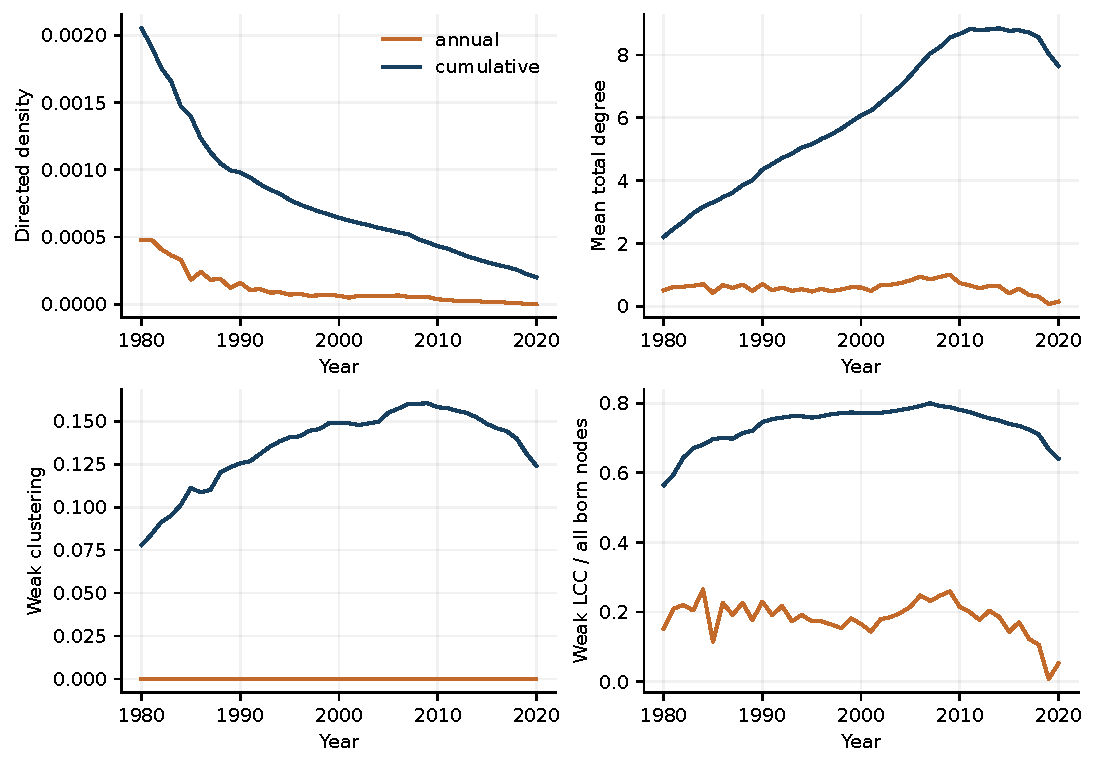
\includegraphics[width=.95\textwidth]{b_aggregation.pdf}
\caption{Measured CIT annual and cumulative structure, including born isolates.
The annual zero clustering is imposed by strict publication-year ordering.}
\label{fig:b-aggregation}
\end{figure*}

\paragraph{Window interpretation.}
\Cref{fig:b-window} shows that longer windows connect a larger fraction of born
papers and admit cross-year triangles. These effects require a sequence of
snapshots; one final aggregate cannot reveal when connectivity appears.
The relative range is a window-sensitivity statistic, not a significance test
against a temporal null, and identical density/degree sensitivity follows from
the common denominator.

\begin{figure*}[t]
\centering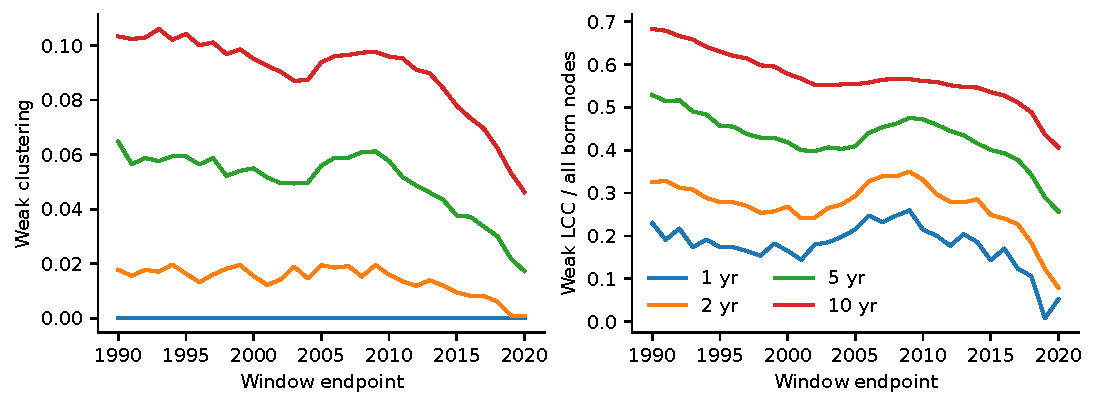
\includegraphics[width=.95\textwidth]{b_window_sensitivity.pdf}
\caption{Measured CIT trailing-window clustering and connectivity for 1, 2, 5
and 10 years. Born isolates are included at every endpoint.}
\label{fig:b-window}
\end{figure*}


\paragraph{Verdict on H1.}
Supported for CIT under the stated node denominator and strict-year convention.
A comparative verdict for PS and CM awaits their measurements; the relative
sensitivity of network types cannot yet be ranked.
